\documentclass[10pt]{article}
\usepackage[paperwidth=7.4in,paperheight=6.9in,margin=0.12in]{geometry}
\usepackage{amsmath,amssymb,bm}
\usepackage{tikz}
\usetikzlibrary{arrows.meta,positioning,calc,fit,backgrounds}
\pagestyle{empty}
\definecolor{inputgray}{RGB}{76,84,92}
\definecolor{predblue}{RGB}{42,104,145}
\definecolor{controlred}{RGB}{181,74,58}
\definecolor{controlorange}{RGB}{196,116,42}
\definecolor{fitpurple}{RGB}{102,75,145}
\begin{document}
\centering
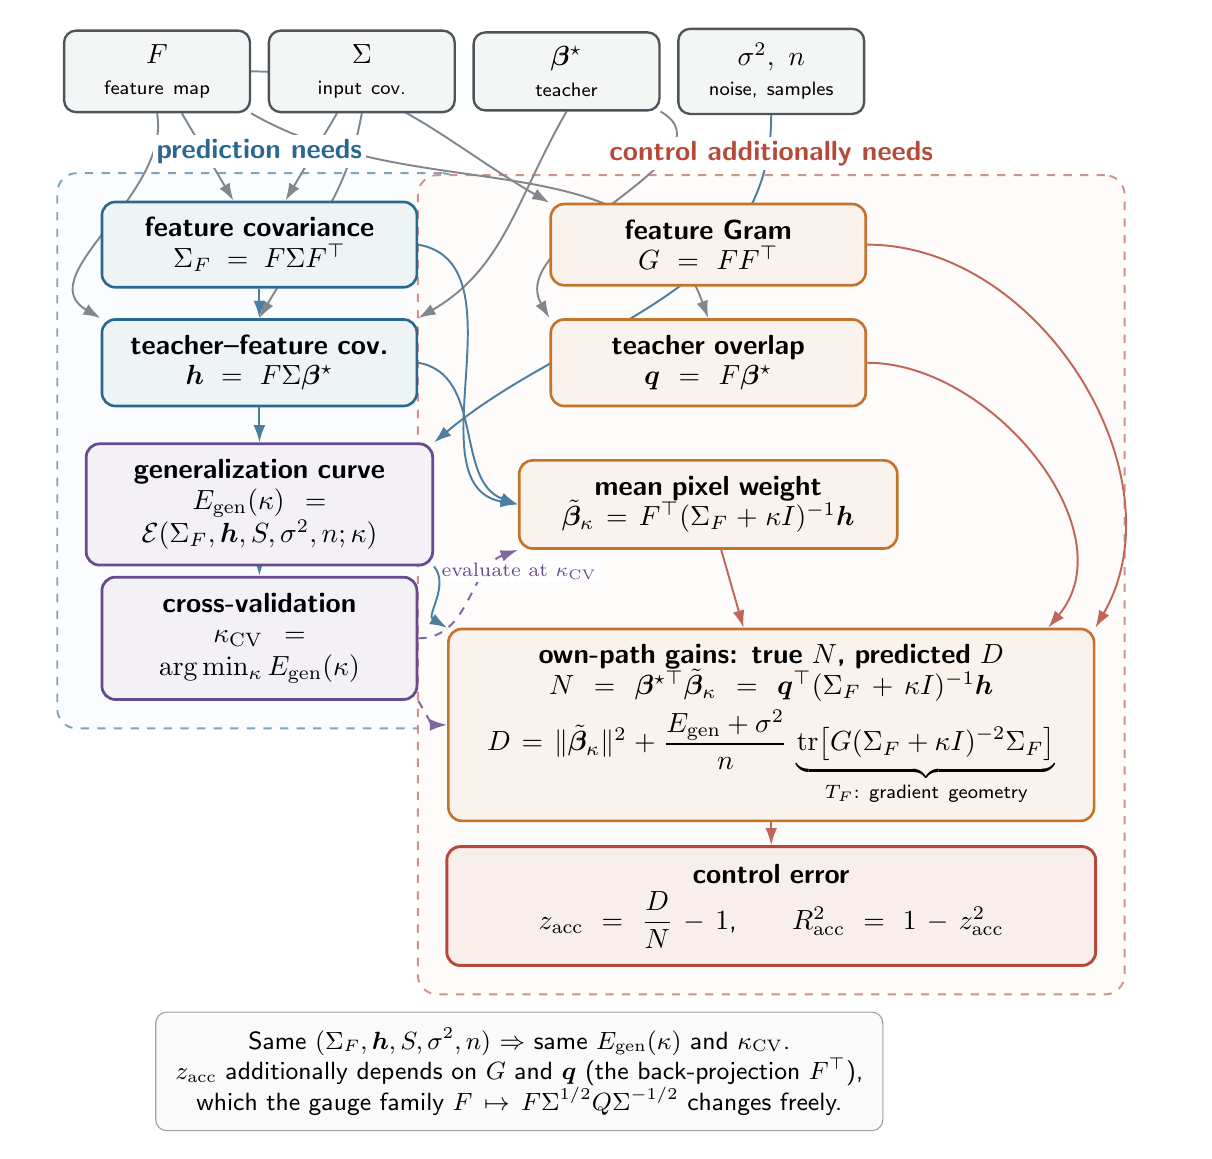
\begin{tikzpicture}[
  x=1cm,y=1cm,font=\sffamily,>=Latex,
  dep/.style={-{Latex[length=2.2mm,width=1.5mm]},draw=inputgray!70,line width=0.7pt},
  pdep/.style={dep,draw=predblue!85},
  cdep/.style={dep,draw=controlred!85},
  kdep/.style={dep,draw=fitpurple!85,dashed},
  input/.style={draw=inputgray,line width=0.85pt,rounded corners=1.5mm,fill=inputgray!6,
                text width=2.0cm,minimum height=0.85cm,align=center,inner sep=1.8mm},
  pstat/.style={draw=predblue,line width=0.95pt,rounded corners=1.7mm,fill=predblue!8,
                text width=3.6cm,minimum height=0.95cm,align=center,inner sep=2mm},
  cstat/.style={draw=controlorange,line width=0.95pt,rounded corners=1.7mm,fill=controlorange!9,
                text width=3.6cm,minimum height=0.95cm,align=center,inner sep=2mm},
  fitbox/.style={draw=fitpurple,line width=1.0pt,rounded corners=1.7mm,fill=fitpurple!8,
              text width=4.4cm,minimum height=0.95cm,align=center,inner sep=2mm},
  cout/.style={draw=controlred,line width=1.05pt,rounded corners=1.7mm,fill=controlred!9,
               align=center,inner sep=2.2mm},
  group/.style={draw,line width=0.7pt,dashed,rounded corners=2.5mm,inner sep=3.5mm}
]
% ---------- inputs (top row)
\node[input] (F)     at (0.0,0)  {$F$\\[-1pt]\scriptsize feature map};
\node[input] (Sigma) at (2.6,0)  {$\Sigma$\\[-1pt]\scriptsize input cov.};
\node[input] (beta)  at (5.2,0)  {$\bm\beta^\star$\\[-1pt]\scriptsize teacher};
\node[input] (noise) at (7.8,0)  {$\sigma^2,\ n$\\[-1pt]\scriptsize noise, samples};
% ---------- prediction column (left)
\node[pstat] (SF)   at (1.3,-2.2) {\textbf{feature covariance}\\[-1pt]$\Sigma_F=F\Sigma F^\top$};
\node[pstat] (h)    at (1.3,-3.7) {\textbf{teacher--feature cov.}\\[-1pt]$\bm h=F\Sigma\bm\beta^\star$};
\node[fitbox,text width=4.0cm] (Egen) at (1.3,-5.5) {\textbf{generalization curve}\\[-1pt]$E_{\rm gen}(\kappa)=\mathcal E(\Sigma_F,\bm h,S,\sigma^2,n;\kappa)$};
\node[fitbox,text width=3.6cm] (kcv) at (1.3,-7.2) {\textbf{cross-validation}\\[-1pt]$\kappa_{\rm CV}=\arg\min_\kappa E_{\rm gen}(\kappa)$};
% ---------- control column (right)
\node[cstat] (G)  at (7.0,-2.2) {\textbf{feature Gram}\\[-1pt]$G=FF^\top$};
\node[cstat] (q)  at (7.0,-3.7) {\textbf{teacher overlap}\\[-1pt]$\bm q=F\bm\beta^\star$};
\node[cstat,text width=4.4cm] (bt) at (7.0,-5.5) {\textbf{mean pixel weight}\\[-1pt]$\tilde{\bm\beta}_\kappa=F^\top(\Sigma_F+\kappa I)^{-1}\bm h$};
\node[cstat,text width=7.8cm] (ND) at (7.8,-8.3)
  {\textbf{own-path gains: true $N$, predicted $D$}\\[-1pt]
   $N=\bm\beta^{\star\top}\tilde{\bm\beta}_\kappa=\bm q^\top(\Sigma_F+\kappa I)^{-1}\bm h$\\[2pt]
   $D=\|\tilde{\bm\beta}_\kappa\|^2+\dfrac{E_{\rm gen}+\sigma^2}{n}\,\underbrace{\operatorname{tr}\!\big[G(\Sigma_F+\kappa I)^{-2}\Sigma_F\big]}_{T_F:\ \text{gradient geometry}}$};
\node[cout,text width=7.8cm] (z) at (7.8,-10.6)
  {\textbf{control error}\\[2pt]$z_{\rm acc}=\dfrac{D}{N}-1$,\qquad $R^2_{\rm acc}=1-z_{\rm acc}^2$};
% ---------- groups and arrows
\begin{scope}[on background layer]
  \node[group,draw=predblue!60,fill=predblue!2,fit=(SF)(h)(Egen)(kcv)] (pg) {};
  \node[group,draw=controlred!60,fill=controlred!2,fit=(G)(q)(bt)(ND)(z)] (cg) {};
  \draw[dep] (F) -- (SF);   \draw[dep] (Sigma) -- (SF);
  \draw[dep] (F.south) to[out=-80,in=150] (h.north west);  \draw[dep] (Sigma.south) to[out=-100,in=60] (h.north);   \draw[dep] (beta.south) to[out=-120,in=30] (h.north east);
  \draw[dep] (F.east) to[out=0,in=150] (G.north west);
  \draw[dep] (beta.south east) to[out=-30,in=120] (q.north west);
  \draw[dep] (F.south east) to[out=-30,in=110] (q.north);
  \draw[pdep] (SF) -- (h);  \draw[pdep] (h) -- (Egen);
  \draw[pdep] (noise.south) to[out=-90,in=40] (Egen.north east);
  \draw[pdep] (Egen) -- (kcv);
  \draw[kdep] (kcv.east) to[out=0,in=-160] (bt.south west);
  \node[font=\scriptsize,text=fitpurple,fill=white,inner sep=1pt] at (4.6,-6.35) {evaluate at $\kappa_{\rm CV}$};
  \draw[kdep] (kcv.south east) to[out=-60,in=180] (ND.west);
  \draw[pdep] (SF.east) to[out=-10,in=170] (bt.west);
  \draw[pdep] (h.east) to[out=-10,in=160] (bt.west);
  \draw[cdep] (G.east) to[out=0,in=60] (ND.north east);
  \draw[cdep] (q.east) to[out=0,in=50] ([xshift=-6mm]ND.north east);
  \draw[cdep] (bt) -- (ND);
  \draw[pdep] (Egen.south east) to[out=-50,in=150] (ND.north west);
  \draw[cdep] (ND) -- (z);
\end{scope}
\node[font=\bfseries\sffamily,text=predblue,fill=white,inner sep=1.5pt,anchor=south] at ([yshift=0.5mm]pg.north) {prediction needs};
\node[font=\bfseries\sffamily,text=controlred,fill=white,inner sep=1.5pt,anchor=south] at ([yshift=0.5mm]cg.north) {control additionally needs};
\node[draw=inputgray!55,fill=black!2,rounded corners=1.4mm,text width=9.0cm,align=center,inner ysep=2.0mm,font=\small\sffamily]
  at (4.6,-12.7)
  {Same $(\Sigma_F,\bm h,S,\sigma^2,n)$ $\Rightarrow$ same $E_{\rm gen}(\kappa)$ and $\kappa_{\rm CV}$.\\
   $z_{\rm acc}$ additionally depends on $G$ and $\bm q$ (the back-projection $F^\top$),\\ which the gauge family $F\mapsto F\Sigma^{1/2}Q\Sigma^{-1/2}$ changes freely.};
\end{tikzpicture}
\end{document}
